%
% File coling2014.tex
%
% Contact: jwagner@computing.dcu.ie
%%
%% Based on the style files for ACL-2014, which were, in turn,
%% Based on the style files for ACL-2013, which were, in turn,
%% Based on the style files for ACL-2012, which were, in turn,
%% based on the style files for ACL-2011, which were, in turn, 
%% based on the style files for ACL-2010, which were, in turn, 
%% based on the style files for ACL-IJCNLP-2009, which were, in turn,
%% based on the style files for EACL-2009 and IJCNLP-2008...

%% Based on the style files for EACL 2006 by 
%%e.agirre@ehu.es or Sergi.Balari@uab.es
%% and that of ACL 08 by Joakim Nivre and Noah Smith

\documentclass[11pt]{article}
\usepackage{coling2014}
\usepackage{times}
\usepackage{url}
\usepackage{latexsym}
\usepackage{hyperref}
\usepackage{todonotes}
\usepackage{textcomp}
\usepackage{graphicx}
\graphicspath{ {images/} }
%\setlength\titlebox{5cm}

% You can expand the titlebox if you need extra space
% to show all the authors. Please do not make the titlebox
% smaller than 5cm (the original size); we will check this
% in the camera-ready version and ask you to change it back.

\newcommand{\TODO}[1]{\todo[inline]{{\footnotesize #1}}}

\title{Title}

\author{First Author \\
  Affiliation / Address line 1 \\
  Affiliation / Address line 2 \\
  Affiliation / Address line 3 \\
  {\tt email@domain} \\\And
  Second Author \\
  Affiliation / Address line 1 \\
  Affiliation / Address line 2 \\
  Affiliation / Address line 3 \\
  {\tt email@domain} \\}

\date{}

\begin{document}
\maketitle
\begin{abstract}
Abstract
\end{abstract}

\TODO{add todos and comments wherever you like, like this!}

\section{Introduction}
\subsection{Positive things about AVs}
Soon(/Already) traversing the streets of "relevant place" the future of autonomous vehicles is coming closer to being a part of today's reality. The dream of self driving cars holds many promises, with one of it's bigger points being safety.

In 2011 more then 2.2 million injuries were caused from automobile crashes in the United States alone \cite[p. 14]{Anderson2014rand}, while more then 39 percentage of all fatalities involved alcohol\cite[p. 16]{Anderson2014rand}. With a far greater field of vision, reaction time and control of safety-critical functions, the hopes is that autonomous vehicles could drastically reduce these statistics.

It's possible that the group most influenced by the self driving cars are the people that are not capable of driving themselves. For these groups the self driving cars could higher convenience, reliability and personal independence \cite[p. 17]{Anderson2014rand}.

More efficient and aware driving in addition to the possibilities of higher space efficiency due to the heightened safety could vastly reduce fuel consumption and CO$_2$ emissions \cite[p. 28ff]{Anderson2014rand}.

\subsection{History}
... in 1926 a driverless car drove the streets of Milwaukee. At the time the technology used to make this work was to radio-controll the car from a following car. 
Radio-controlled cars ~1920\\
%TODO \cite{The Milwaukee Sentinel:26}\\ 
Curciuts, wires and devices imbedded in the roadway ~1930-1960\\
%TODO \cite{Press-Courier:60}\\ 
Neural Networks ~1990\\
95-98\% autonomous ~1990\\
DARPA / DARPA Grand Challenge ~2000\\
\cite{Thrun2006stanley}\\
Early 2014 the first self driving car Navia 
Autonomous cars on the roads ~2010\\
%TODO \cite{eWeek:14}


\section{How AVs work}
\subsection{Sensors}
In order for the autonomous vehicles to navigate the real world, its software needs to obtain data about itself and its surroundings. For that purpose, AVs have several types of sensors incorporated to its body. The software processes the data provided by those sensors to create a virtual representation of the real world which can then use to calculate which actions to take to reach its destination. There are two main types of sensors: Exterioceptive and proprioceptive. The former deals with information from the AV's environment, while the later deals with information internal to the system. Some examples of the data that can be obtained within each class are:
\begin{itemize}
	\item Extereoceptive: Distances to objects, object types, objects' speed and heading.
	\item Proprioceptive: Motor speed, wheel load, heading, position, battery status.
\end{itemize}
For a more functional perspective, the sensors can be organized into categories defined by its use cases for AVs:
\begin{itemize}
	\item \textbf{Know where you are going}:
		\begin{itemize}
			\item \textbf{GPS}: It allows the AV to determine its position in absolute terms. In optimal conditions it has good accuracy and precision. It cannot be constantly relied upon due to intermittent coverage caused by tunnels, canyons, buildings, radio interference, etc.
			\item \textbf{IMU}: A type of dead-reckoning system using a 3-axis accelerometer and a 3-axis gyroscope. It provides data on linear and rotational motion, which is then used to calculate the motion and relative position of the vehicle regardless of any sort of signal obstruction. It has good accuracy for short periods but has cumulative error so over time it gets very inaccurate.
			\item \textbf{Compass}: It can be used to determine the AV's heading. It has good accuracy which doesn't change over time but it is subject to interference by magnetic objects and electrical sources. It also can be slow to settle except for the most expensive types.
			\item \textbf{Ground speed RADAR}: Measures real ground speed using the Doppler effect. It can be used for dead-reckoning.
			\item \textbf{Wheel odometry}: Used for dead reckoning. Uses optical encoders to measure the speed of the wheels and the direction of the steering wheel from which the relative position of the AV can be calculated.
		\end{itemize}
	\item \textbf{See where you are going}:
		\begin{itemize}
			\item \textbf{LIDAR}: The device emits laser pulses, and measures the time the beam takes to reflect back to the sensor (Time-of-flight), then it calculates the distance using that measurement. By using a rotating, scanning mirror assembly on top of the AV, it provides 3D 360{\textdegree} view suitable for ``big picture'' imaging. It is not very effective for close-in control.
			\item \textbf{Cameras}: They are typically used to enhance the resolution of the 3D information obtained by the LIDAR, as well as detecting street signs and road markings. Its effectivness is affected by reduced visibility conditions such as dusk, bad weather and dirt on the lens.
			\item \textbf{RADAR}: Similar to LIDAR but instead of laser it uses a normal radio wave beam (usually 77GHz) to measure distance. It is used for close-in control instead of LIDAR: Parking, lane-changing and bumper-to-bumper traffic.
		\end{itemize}
	\item \textbf{Get where you are going}:
		Other sensors are needed for the correct operation of the AV, which deal with the internal state of the vehicle, such as: Battery \& fuel level sensors, engine temperature, oil pressure, etc.
\end{itemize}

\subsection{Software}
Cars create very specific maps
    maps take into account everything around them
    cars send back data they collect to update location map information
Cars figure out where they are by finding where they fit on the map, much like if you had a section of a map you could fit it in the context of the entire map
software maps all things around the car
looks at cyclysts, pedestrians, other cars, solid objects
Also trafic cones, people in vests, etc. 
Anticipates what each thing is going to do and when. 
Readjusts bases on what actually happens 
If it is not sure of something it slows to a stop
\par
In order to use the sensors to actually drive humans need to program how to interpret all the data the sensors collect. The main concerns of the car is driving, and avoiding all other objects. 
The cars use the sensors to figure out where they are. Google has created very specific maps for the cars to use to find there location. These maps include everything about an area including curb height, intersection width, and lane layout. 
The cars figure out where they are by matching the images from the sensors to
a specific place on the map. They use where the car was a few seconds prior to help them make location matches in real
time. The reason they use this complicated mapping system instead of a more common GPS system is because GPS is not
acurate enough. Moreover GPS systems can lose conection because of tall buildings and is not acurate enough to
consistantly figure out what side of the road a car is on. However the preinstalled maps also have issues. For one the
cars are not able to drive in snow because the snow changes the landscape and therefore the physical markers google
usually uses to place a car. While the cars rely on the maps immensily it knows that roads do change. They are
constantly sendind data back to google about changes in roads because of errosion or construction. \par
After the cars figure out exactly where they are they need to then worry about cars, pedestrians, workers, and cyclists.
Within those catigories there is more specific catigorizations. For example the cars differinatiate between, trucks or
road worker in orange vests. They also look out for common things in the road like traffic cones. Once they recognize
that there is something it is usually hard to figure out exactly what it is. The computers use machine learning to
differentiate between every possibility. As you can see in the image below the car maps 
\begin{figure}[!ht]
  \centering
      \reflectbox{%
                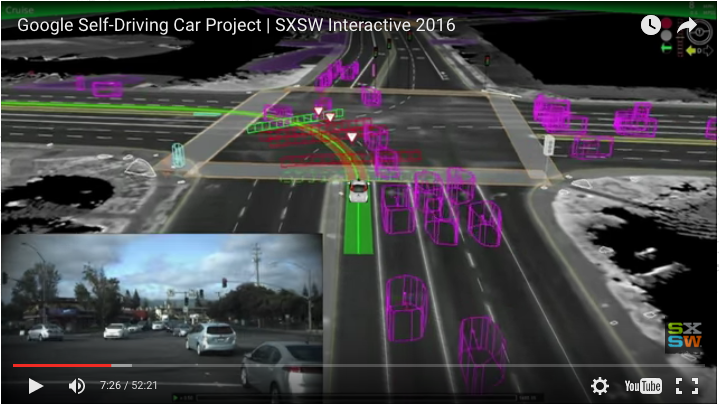
\includegraphics[width=0.7\textwidth]{drivingcar}}
                  \caption{The small box to the left is a picture from the front window of the car. The rest of the
                      image is how the car interperets images from the sensors. The purple boxes are other motered
                          veichals. The blue box on the crosswalk is a person. The green track is where the car has to
                          go. The long green and red cylinders and the projected motion of cars that would end up in the
                  path of the car.}
\end{figure}

\par


\section{Social and Ethical Implications of AVs}
\TODO{Gerd: I'm pretty sure this is more than enough material for this section already. If we include all the bullet points I listed here, I will not be able to go into any detail (which is what we want?)}.

\subsection{Everyday Life and Social Implications}
%TODO \cite{Rand:16}
\begin{itemize}
\item most likely \textbf{changed patterns of land use}: low-density patterns of land-use surrounding metropolitan regions due to facilitated mobility.
\item \textbf{Mobility for those unable or unwilling to drive}: independence, reduction of social isolation, ... possibly connect this to the gap between rich and poor.
\item \textbf{Free time}: Time spent in an AV could be used as work time or free time to a certain extent.
\item \textbf{Energy and emissions}: the overall effect is unclear, total VMT will likely increase, but the technology offers the possibility to decrease emissions as well. 
\end{itemize}

\subsection{Economics}
Many jobs and a variety of professions will likely be affected by the introduction of AVs. In 2015, rougly 1.18 million bus and truck drivers have been employed in the US according to the Bureau of Labor Statistics \cite{USLabourBureau}, and those are only two examples of professions which would be affected in a very direct way. Decreasing crash risks could impair the business of many insurance companies, and since AVs could facilitate the introduction of alternative fuels, jobs related to combustion enginges might become obsolete. According to \cite[p. 40ff]{Anderson2014rand}, ``... lost jobs might be replaced by others, perhaps related to the AV industry, but there may be considerable economic disruption''. Not only technical solutions necessary here, but also appropriate policy reactions and extensive discussion and changes in society. The introduction of an unconditional basic income is a possible reaction to increasing automatoin that is currently being discussed controversialy. \todo{add literature reference here, e.g. ``rise of the machines'' paper?}
AVs will, just like most state-of-the-art technology, likely be very expensive in the first years. Thus, this presumably safe, fast, reliable and convenient mean of transportation might be only available to the richer parts of the population. Driving conventional cars could become a necessity for the poor, further increasing the social gap between rich and poor. Compare \cite[p. 39]{Anderson2014rand}.

\subsection{Legal}
\begin{itemize}
\item \textbf{Liability implications}: The manufacturer's liability will likely increase (danger of slowdown of technology adoption - possible discussion: how big a danger is this?). This might lead to \textbf{vehicles as a service}. \textbf{Closer monitoring of driver behaviour} is mentioned in the RAND report as well, this might be a point of discussion.
\item \textbf{Policy toolkit}: federal insurance backstop, or simply assign liability to human drivers? \textit{tort preemption??}
\end{itemize}

\subsection{Ethical Issues}
\begin{itemize}
\item Automated vehicles would almost certainly crash
\item An automated vehicle's decisions that preceded certain crashes has a moral component. 
\item There is no obvious way to encode complex human morals effectively in software. 
\end{itemize}
\cite{Goodall2014ethical}

\subsubsection{Possible AV ethics approaches}

\begin{itemize}
\item \textbf{Rational Approaches}. Deontology (AV must adhere to a set of rules), consequentialism (system's goal is to maximize some benefit). \textbf{Problems}: Incompleteness of any set of rules and the difficulty involved in the articulation of complex human ethics as a set of rules.
\item \textbf{AI Approaches}. Idea: Train a neural network on a combination of simulations and recordings of real crashes, with human feedback on the ethical response. \textbf{Problems}: Inconsistency between how humans actually behave and what they believe, and lacking traceability (why did the NN decide the way it did?? Risk of missing transparency and manipulation).
\end{itemize}

\subsubsection{Proposed Ethical Vehicle Deployment Strategy}
Analogy: moral education of a child.
\begin{enumerate}
\item Phase 1: Rational Ethics
\item Phase 2: Hybrid rational and AI approach (rule system from Phase 1 should remain in place as boundary)
\item Phase 3: Feedback with Natural Language (active field of research)
\end{enumerate}

\section{Conclusion}
\subsection{Future of AVs}
...
\subsection{Our Predictions}
\begin{itemize}
\item Gerd: lost jobs and professions will be a huge challenge for our society. 
\end{itemize}


\TODO{Gerd: I created a BibTex bibliography file (Bibliography.bib), and added the bibtex code for some of our references. Now this has to be done for the other references as well. I moved the old bibliography code to OldBibliography.tex until we've entirely switched to bibtex. You can usually find the complete BibTex code for most books and articles by simply googling the title + ``bibtex'' or by using google scholar and pressing the ``cite'' button there.}

\TODO{Another hint: you might have to delete all the temporary files in the folder (.aux, .bbl), and compile the document two or three times before the actual references are correctly inserted into the document instead of only question marks.}

% BibTeX 
\TODO{Switching to IEEETran bibstyle currently causes errors.}
%\bibliographystyle{IEEEtran}
\bibliographystyle{acl}
%\bibliography{acl2014}
\bibliography{Bibliography}


\end{document}

%%% Local Variables:
%%% mode: latex
%%% TeX-master: t
%%% End:
